\begin{figure*}[h]
	\centering
	\begin{minipage}[b]{0.45\linewidth}
		\centering
		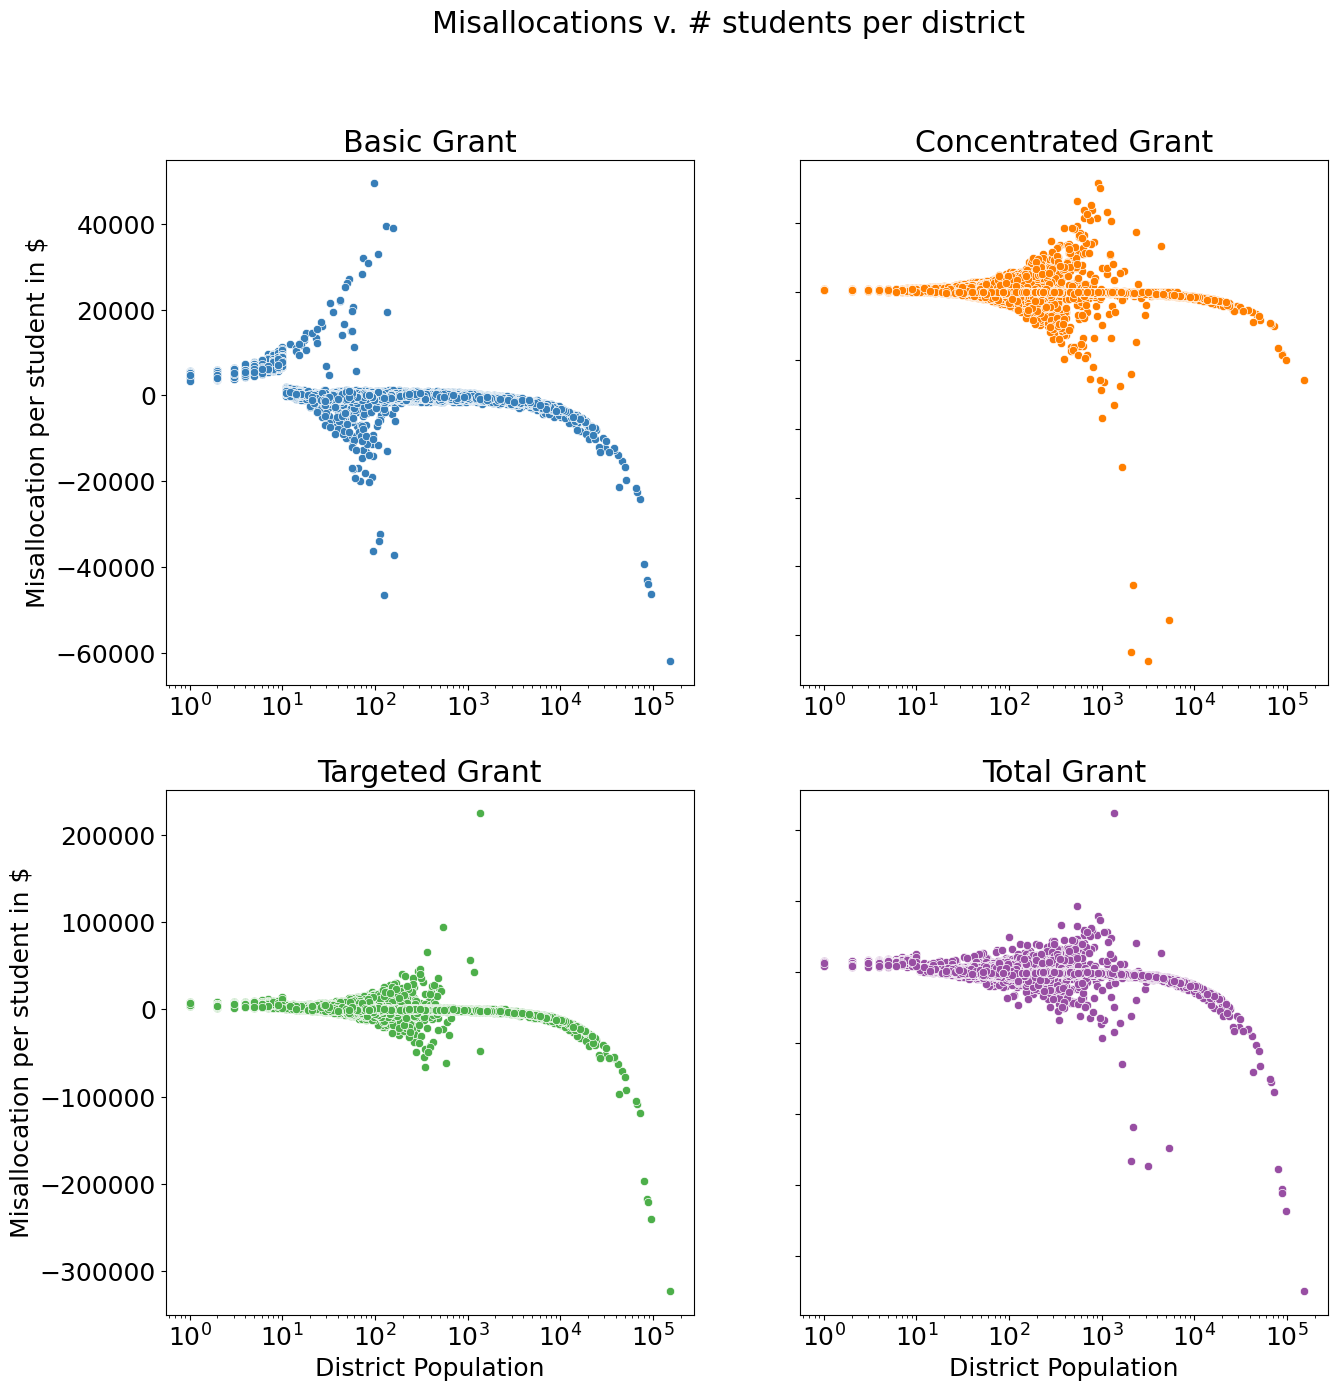
\includegraphics[width=\linewidth]{images/all_grant_errors_total}
		\caption{Misallocations in USD compared to district size}
		\label{fig:misalloc_total}
	\end{minipage}
	\hfill
	\begin{minipage}[b]{0.45\linewidth}
		\centering
		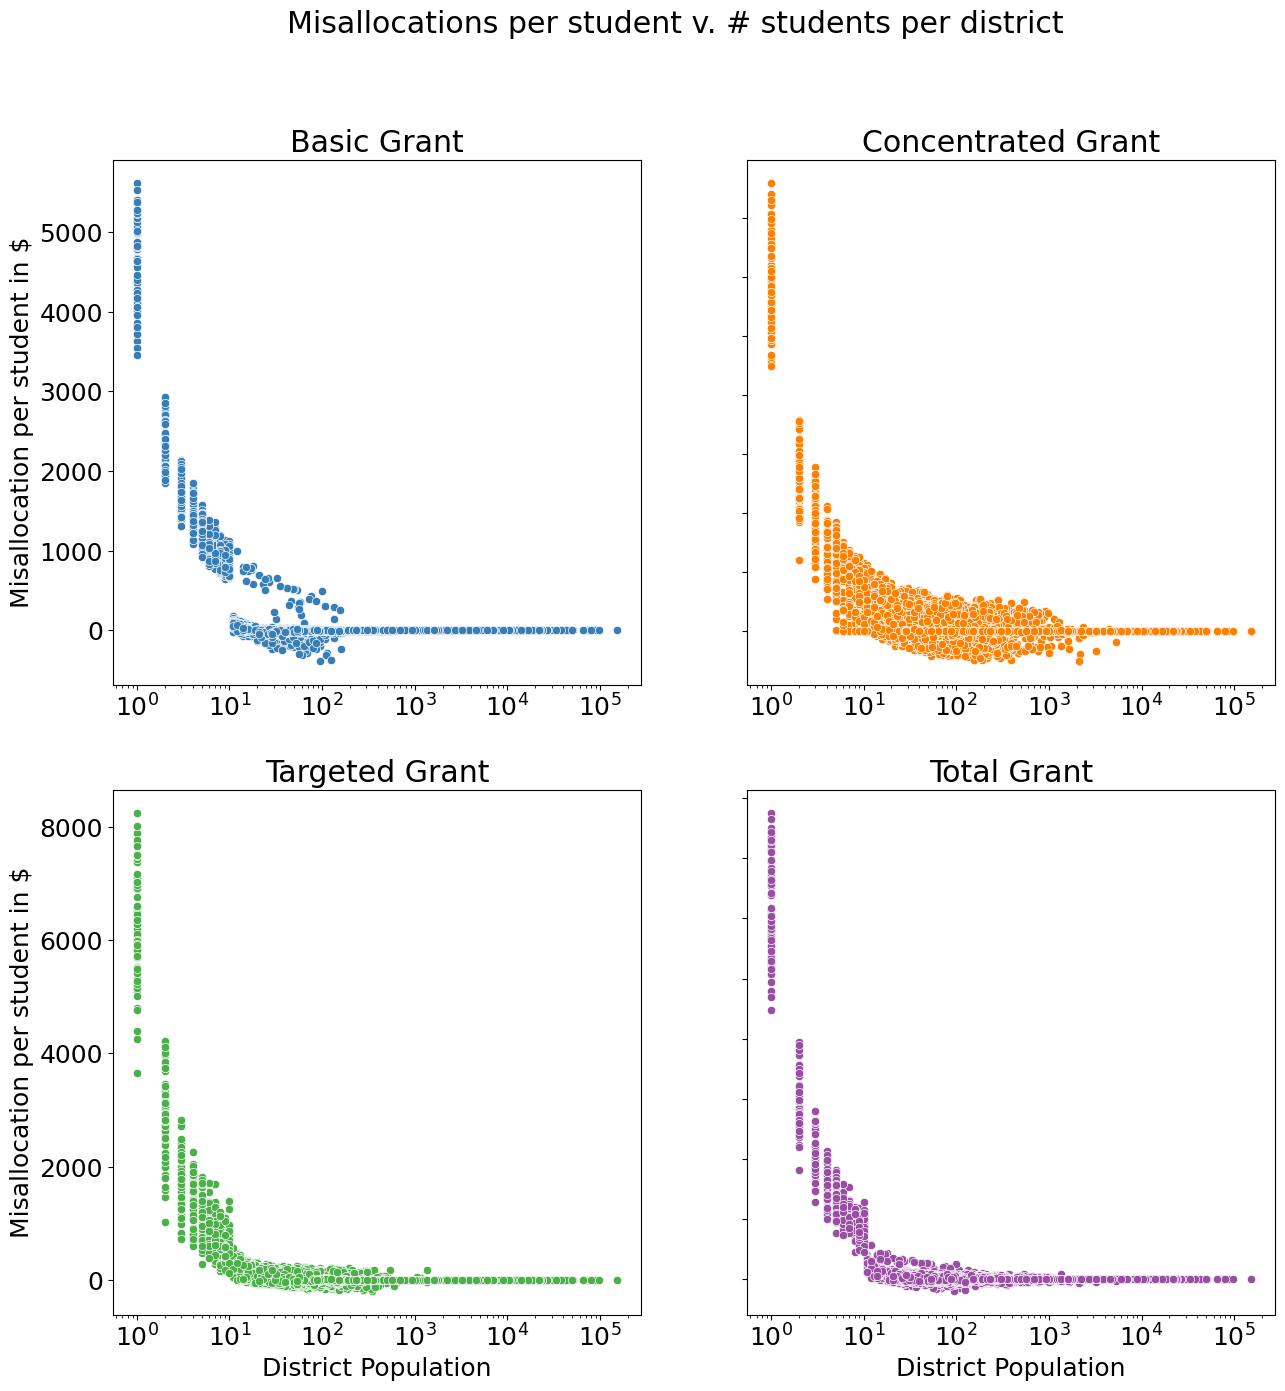
\includegraphics[width=\linewidth]{images/all_grant_errors_per_capita}
		\caption{Misallocations in USD per student compared to district size}
		\label{fig:misalloc_per_student}
	\end{minipage}
	\caption{We apply differential privacy with a privacy budget of $\rho=2.65$ to the population and eligible
	population counts of each district. We then plot the Title I misallocations for each district in the US for the
	basic, concentrated, and targeted grants, calculated using the allocation formulas outlined in \cite{Sonnenberg:16}.
	We observe that while large districts are more likely to receive larger misallocations, smaller districts are more
	likely to receive larger misallocations per student. We attribute these results to the complex interaction
	between differential privacy and the thresholds in the allocation formulas.}
	\label{fig:misalloc_comparison}
\end{figure*}

